\documentclass[a4paper,11pt,oneside,%twoside to print on the back of pages
headsepline,												% Linie für Kopfzeile
footsepline,												% Linie für Fußzeile
bibtotocnumbered									% numb point literaturverz in inhaltsverz => bibliography=tot ocnumbered
]{scrreprt}
%----------------------------------------------------------------------------------------------------------------------------------------------
% STANDART LIBS
\usepackage[T1]{fontenc}
\usepackage[utf8]{inputenc}
\usepackage[ngerman]{babel}    % Deutsche Sprache in automatisch generiertem

% DRUCKBEREICH: \areaset[BCOR]{textwidth}{textheight} %TODO understand
% BCOR ist "Binding Correction", also wieviel Innenrand verloren geht
% A4 hat 297mm x 210mm
% wenn keine Marginalien, dann ist Breite 15cm vielleicht besser
\areaset[1.5cm]{14cm}{25cm} 
%% Die folgende Zeile sorgt dafür, daß die Fußnoten eingerückt werden,
%% und zwar um 2em (class scrbook).
\deffootnote{2em}{2em}{\textsuperscript{\normalfont\thefootnotemark} }

%----------------------------------------------------------------------------------------------------------------------------------------------
% ADDITIONAL LIBS



% Wrapping text around figures
\usepackage{wrapfig}  %
% containers for things that cannot be broken over a page -> example table, figure
\usepackage{float}
% provides many ways to customise the captions in floating environments
\usepackage{caption} % http://www.ctex.org/documents/packages/float/caption.pdf
% same for subfigues
\usepackage{subcaption} % hint include subpicture

%% Unterstützung für Graphiken und Farben
\usepackage[pdftex]{graphicx}
%\usepackage[pdftex]{color}
%\definecolor{DSblue}{rgb}{0,0,0.9}   % example defining a color



% INDEX/GLOSSARY %TODO
%Defines commands for use with MakeIndex
%\usepackage{makeidx} % -> en.wikibooks.org/wiki/LaTeX/Indexing pctex.com/files/managed/3/3a/makeindx.pdf
%\usepackage[xindy,toc]{glossaries}
\usepackage{acronym} %Abkürzungsverzeichniss

%BIBTEX
%used by biblatex for qutes
\usepackage[babel,german=quotes]{csquotes} % load after inputenc
% cite package -> 1. pdflatex xx.tex 2. biber xx 3. pdflatex xx.tex
\usepackage[style=reading,backend=biber]{biblatex} %TODO check diff cite styles
% loads the bib file
\addbibresource{bachelorBib.bib}


% cross referencing and hyperrefs
\usepackage[                % FIXME explain
   pdftex,                  % Ausgabe-Medium: PDF
   colorlinks=true,         % farbige Links in der Bildschirm-Version?
   pdfstartview=Fit,       % wie soll Acrobat starten?
   linkcolor=black,         % Farbe für Querverweise
   citecolor=black,         % Farbe für Zitierungen
   urlcolor=black,          % Farbe für Links
   bookmarks=true
   ]{hyperref}
% non clickable URL   		
\usepackage{url} %TODO remove if hyperref is better

% TODONOTES -> http://tex.stackexchange.com/questions/9796/how-to-add-todo-notes
\usepackage{lipsum}                     % Dummytext
\usepackage{xargs}                      % Use more than one optional parameter in a new commands
\usepackage[pdftex,dvipsnames]{xcolor}  % Coloured text etc.
% -> www.tex.ac.uk/ctan/macros/latex/contrib/todonotes/todonotes.pdf
\usepackage[colorinlistoftodos,prependcaption,textsize=tiny]{todonotes}
\newcommandx{\unsure}[2][1=]{\todo[linecolor=red,backgroundcolor=red!25,bordercolor=red,#1]{#2}}
\newcommandx{\change}[2][1=]{\todo[linecolor=blue,backgroundcolor=blue!25,bordercolor=blue,#1]{#2}}
\newcommandx{\info}[2][1=]{\todo[linecolor=OliveGreen,backgroundcolor=OliveGreen!25,bordercolor=OliveGreen,#1]{#2}}
\newcommandx{\improvement}[2][1=]{\todo[linecolor=Plum,backgroundcolor=Plum!25,bordercolor=Plum,#1]{#2}}
\newcommandx{\thiswillnotshow}[2][1=]{\todo[disable,#1]{#2}}

% Print graphics
% tikz print graphs: http://www.texample.net/tikz/examples/
% bytefield – Create illustrations for network protocol specifications

% source code include
\usepackage{listings} % -> %TODO use minted
\usepackage{minted}

%----------------------------------------------------------------------------------------------------------------------------------------------
% ADDITIONAL LIBS TO CHECK

%linien in Tabellen
\usepackage{booktabs}
\usepackage{anysize}
\usepackage[onehalfspacing]{setspace}


% math for matrix and $$
%\usepackage{amsmath}
%\usepackage{amssymb}

%\usepackage{lmodern}

%\usepackage{multido}    % FIXME ???????????
%\usepackage{everysel}   % FIXME ???????????
 
%% besserer Flattersatz: \RaggedRight
\usepackage{ragged2e}

% from exposee
\usepackage{latexsym}         % Fuer recht seltene Zeichen

\usepackage[a4paper,lmargin={2.5cm},rmargin={2.5cm},tmargin={3cm},bmargin={2.5cm}]{geometry}
\usepackage{enumerate}

\newcommand{\HRule}{\rule{\linewidth}{0.5mm}}

\pdfinfo{
	/Title		(Synchronisation von Binärbaum-indexierten, verteilten InMemory-NoSQL-Datenbanken)
	/Subject		(Bachelorarbeit)
	/Author		(Paul Kitt)
}
%----------------------------------------------------------------------------------------------------------------------------------------------
\pagenumbering{roman}
\begin{document}

%TODO set 1,5 zeilenabstand , verdana, schriftgroesse 10
%TODO style titelSeite -> check jonny -> richtliene
%TODO check bewilligten title 
\title{{\bf Bachelorarbeit:} \\ \begin{large}Synchronisation von Binärbaum-indexierten, verteilten
InMemory-NoSQL-Datenbanken\end{large}}
\author{
	Paul Kitt \\
	528516   \\	
	paul.kitt@student.htw-berlin.de	\\
\\
\textbf{Studienort:}	\\
	Hochschule für Technik und Wirtschaft Berlin \\
	Angewandte Informatik (FB4) \\
	\textbf{Betreuer:} \\
	Prof. Dr.-Ing. Hendrik Gärtner, HTW Berlin \\
	Jens-Peter Haack,  SpinningWheel GmbH
}

\begin{titlepage}
	\begin{center}
		\begin{figure}[!htb]
			\minipage{0.5\textwidth}
				\begin{center}
			  		
\includegraphics[width=0.5\textwidth]{bilder/htwLogo.jpeg}
				\end{center}
			\endminipage\hfill
		 	\minipage{0.5\textwidth}
				\begin{center}
			 		
\includegraphics[width=0.5\textwidth]{bilder/Spinning_O_Wheel-200.png}
				\end{center}	
			\endminipage
		\end{figure}
	
		 \vfill
		 \HRule \\[0.4cm]
	    {\bfseries\Large
	        \begin{LARGE}
	        Bachelorarbeit:\\
	        \end{LARGE} 
	        Synchronisation von Binärbaum-indexierten, verteilten
			InMemory-NoSQL-Datenbanken\\
	    }    
		\HRule \\[1.5cm]
	 	\vfill
	
	% Author and supervisor
		\begin{minipage}{0.4\textwidth}
			\begin{flushleft} \large
				\textbf{Author:}\\
				Paul Kitt, 528516 \\
				Angewandte Informatik (FB4) \\	
				Hochschule für Technik und Wirtschaft Berlin\\
				paul.kitt@student.htw-berlin.de	\\~\\
				\textbf{Studienort:}	\\
				Hochschule für Technik und Wirtschaft Berlin \\
				Angewandte Informatik (FB4) \\
			\end{flushleft}
		\end{minipage}
		\begin{minipage}{0.4\textwidth}
			\begin{flushright} \large
				\textbf{Betreuer:} \\
				Prof. Dr.-Ing. Hendrik Gärtner, HTW Berlin \\
				Jens-Peter Haack,  SpinningWheel GmbH
			\end{flushright}
		\end{minipage}	
		\vfill
		\HRule \\
		\begin{minipage}{0.4\textwidth}
			\begin{flushright} \large
				Datum/Unterschrift des Studenten
			\end{flushright}
		\end{minipage}
		\vfill
		{\large \today}
	\end{center}
\end{titlepage}
\tableofcontents
\newpage
%\todo[inline]{table of table}
%\todo[inline]{table of listings}
Abkürzungsverzeichniss:\\
\begin{acronym}[EB-Baum] % option laengest abk def einzuglänge
 	\acro{EB-Baum}{Elastische Binär Baum}
 	\acrodefplural{EB-Baum}[EB-Bäume]{Elastische Binär Bäume}
\end{acronym}
\renewcommand\listoflistingscaption{Verzeichnis aller Codebeispiele}
\listoflistings

	%---------------------------------------------------------------------------------------------------------------------------------------------------	
\chapter{Einleitung}
\pagenumbering{arabic}
\todo[inline]{Hintergrund, größerer Rahmen, kurze Aufgabenstellung}
 		\begin{enumerate}[1.]
			\item  Problemstellung und Motivation
			\item Zielsetzung
			\item Rahmen und Aufbau der Arbeit
		\end{enumerate}
		
	Mögliche Punkte:
	-> Motivation
	-> Aufgabenbeschreibung
	-> Inhalt und Aufbau der Arbeit	
		
	%---------------------------------------------------------------------------------------------------------------------------------------------------	
\chapter{Grundlagen}
\todo[inline]{	theoretische Grundlagen, Beschreibung von Systemen(nur insoweit, als das diese Grundlagen und Beschreibungen unbedingt für das Verständnis erforderlich sind und nicht als bei studierten Informatikern vorausgesetzt werden kann)}

	\begin{enumerate}[1.]
			\item Grundlagen verwendeter Algorithmen
				\begin{enumerate}[1.]
					\item Binär Bäume
					\item Elastische Binär Bäume
				\end{enumerate}
			\item Definition von Begriffen
				\begin{enumerate}[1.]
					\item Verteilung
					\item Synchronisation
					\item NoSql -> CAP, ACID theoreme die meine db erfüllt 
				\end{enumerate}
			\item Grundlagen Datenbanken (Verteilung, Synchronisation)
				\begin{enumerate}[1.]
					\item MySql
					\item NoSql 
					\item Baumbasierter Indexe
				\end{enumerate}
	\end{enumerate}

\section{Elastische Binär Bäume}
\label{sec:ebTreeGrundlagen}
Bei den \enquote{Elastischen Binär Bäumen} handelt es sich um speziell optimierte Variante der \enquote{Binären Suchbäume}. Entwickelt wurden das Konzept von Willy Tarreau\autocite{Tarreau} im Rahmen einer Forschung zum Thema \enquote{Event-scheduling for user-space network applications} und eignen sich daher auch speziell für Betriebssystem Scheduler, bei welchen schnelles priorisieren nach Zeit oder Dringlichkeit wichtig ist. Daten die mit Binär- oder Ganzahlen, wie Integer oder Long, indexiert sind können in dieser wenig bekannten Datenstruktur sehr effizient verwaltet werden. Dabei ist der \enquote{\ac{EB-Baum}} sehr performant wenn es zu sehr vielen den, Baum verändernden, Operationen, wie: Einfügen, Ändern, Abfragen oder Löschen kommt.\unsure{wie richtig zitieren?}\\
Einfügeoperationen und das Abfragen von Blättern wird in O(log n) bewältigt. Löschen in O(1).\\
Als Ausgangskonzepte dienten bei seiner Entwicklung der \enquote{balanciertem Binär Baum}\unsure{mention red black tree} und des \enquote{Radix Baumes}. Da aber Operationen wie Löschen von Blättern bei einem \enquote{balanciertem Binär Baum} O(log n) kosten und der Baum aber gerade Operationen wie diese möglichst schnell bewältigen soll ein signifikanter Nachteil. Bei den \enquote{Radix Bäumen}, die sich laut dem Entwickler Willy Tarreau\autocite[Absatz Introduction]{Tarreau} im Bezug auf Geschwindigkeit sehr gut eigenen, wird aber im Betrieb das allocieren von Speicher und die damit verbundene \enquote{Garbage Collection} zum Perfomanceproblem.\\
Daher ist der \ac{EB-Baum} eine hybride Form aus beiden um diese Mängel aus zu gleichen. Es handelt sich nicht um einen balancierten Baum, was in besonderen Fällen zu einer schlechteren Leistung als die eines \enquote{balanciertem Binär Baum} führt\unsure{mention example}. Die Blätter sind im Baum von links nach rechts aufsteigend, nach einer Binär- oder Ganzahl(e.g. Integer, Long) sortiert.\\
Eine weitere Besonderheit des \ac{EB-Baum} ist dass seine maximale Höhe durch den Datentyp der Schlüssel bestimmt wird.
So kann beispielsweise ein Baum dessen Schlüssel Werte des Datentypes \enquote{Long} sind maximal 64 Ebenen besitzen da der Datentyp aus 64 Bit besteht. Schlüssel werden durch die Abfolge ihrer Binären Repräsentation adressiert. Der Schlüssel dient hierbei wie eine Art binäre Karte. Begonnen am höchsten gesetzten Bits des Schlüssels und wird der Baum Knoten für Knoten durch laufen und an den Knoten bei einer Null links, bei einer Eins rechts abgebogen bis dass Blatt oder falls dieses nicht vorhanden das am naheliegendste gefunden ist

\subsection{Besonderheiten des Baumes}
Durch die besondere Beschaffenheit des Baumes lassen sich viele Operationen sehr leicht umsetzen wie:
\begin{itemize}
	\item \textbf{Abfragen}
	\begin{itemize}
		\item das Abfragen des ersten und letzten Schlüssels
		\item erlangen des nächst kleineren oder größerem Schlüssel zu einem gegeben Schlüssel
		\item genaues Finden eine Schlüssels
		\item das Finden des ähnlichsten Schlüssels falls dieser nicht enthalten ist
		\item einfaches Abfragen von Bereichen durch ein Prefix
		\item erlangen des vorherigem oder nächstem unterschiedlichen Schlüssel zu einem gegeben Schlüssel
		\item mehrfach auftretende Schlüssel werden immer in ihrer eingefügten Reihenfolge zurück gegeben
	\end{itemize}
	\item \textbf{Einfügen}
	\begin{itemize}
		\item Einfügen mit Duplikaten: Falls ein Werte bereits existiert wird ein Duplikat angelegt
		\item Einfügen von nur einzigartigen Schlüsseln: Falls der Schlüssel vorhanden wird Existierende zurück gegeben
	\end{itemize}
\end{itemize}


\subsection{Aufbau des Baumes}
In dem originalem von Willy Tarreau verfassten Konzept\autocite[Absatz Definitions]{Tarreau} werden die Daten, die Baum hält, in \enquote{EB Knoten}
gespeichert. \enquote{EB Knoten} bestehen aus zwei Teilen:
\begin{itemize}
\item Knoten: verknüpft Blätter sowie anderen Knoten
\item Blatt: ist durch einen Schlüssel adressiert, hält Daten e.g. Referenz auf ein Datenobjekt
\end{itemize}


\begin{wrapfigure}{r}{0.6\textwidth}
  \begin{center}
    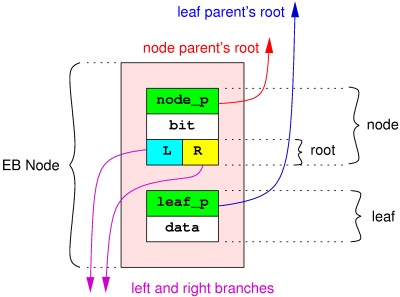
\includegraphics[width=.6\linewidth]{bilder/Ebnode.png}
  \end{center}
 \caption{EB-Knotenelement}
\end{wrapfigure}
Die Aufgabe eines Blattes ist sehr simpel. Es dient nur dazu eingefügte Daten durch einen Pointer zuhalten. Dabei ist es mit einem Schlüssel adressiert und besitzt eine Referenz auf seinen Elternknoten, sowie auf seinen EB-Ursprungsknoten\unsure{SPW fragen}.\\
Ein jedes Knotenelement besteht aus einer Referenz auf sein höher liegenden Elternknoten, dem Ebenenbit \unsure{Darf ich das Bild benutzen?} und zwei Referenzen auf seine Kinderknoten. \\ Das Ebenenbit ist eine Zahl und repräsentiert binär die niedrigste Bitposition des Schlüssels über dem alle Bits gleich sind. Alle unter dem Knoten liegenden Schlüssel haben sich somit bis zu diesem Bit die gleich Bitfolge. Der dritte Teil des Knotens ist die Wurzel die aus zwei Referenzen besteht zu entweder weiteren Knoten oder/sowie Blättern verweist. Da es sich um einen binären Baum handelt repräsentiert je Referenz das linke Bit 0 oder das rechte 1. Nur auf Ebene 0, mit dies repräsentierendem Ebenenbit, kann der Knoten zwei Blätter als Wurzel besitzen, da der Schlüssel sich nur um einen Wert an der letzten, nullten Bitstelle unterscheiden kann.\\
Auch wenn Knoten sich später verschieben können diese nie unterhalb des mit ihnen angefügtem Blattes oder in einen anderen Zweig des Baumes gelangen. Falls es erlaubt ist Duplikate einzufügen werden  Knoten mit negativen Ebenenbits versehen.\\
Eine weitere Besonderheit hier ist dass die Wurzelreferenzen nie unbelegt sind. Nur die Wurzel des Wurzelknoten des Baumes ist hier eine Ausnahme. Wenn seine zwei Wurzeln auf \enquote{null} referenziert ist der Baum leer. Sobald der Baum befüllt wird wächst dieser an seiner linken/\enquote{0-Wurzel}. Die rechte Wurzel referenziert immer auf \enquote{null}. Dadurch lässt sich der der Wurzelknoten einfach erkennen.
Sein Ebenenbit ist die höchste Ebene des Baumes und daher automatisch die binäre Länge des Schlüsseldatentyps, e.g. bei Schlüsseln des Datentyps Long wäre das Ebenenbit 64.\\

\subsection{Einfügen von Daten}
Beim einfügen neuer Datensätze wird jeweils ein Blatt, das die Daten hält, sowie ein Knoten mit dem dass Blatt in Kombination eingefügt wird, eingefügt. Der einzige Fall in dem ein Blatt ohne Knoten angefügt wird ist wenn der Baum leer ist.

Beim Einfügen eines neuen Datensatzes wird ein gesamter \enquote{EB-Knoten} erstellt und an der richtigen Position eingefügt. Werden später weitere Werte gespeichert wird bei deren sortiertem einfügen der Baum umstrukturiert. Dies hat zur Folge dass Knoten und Blatt eines vorher übereinander liegenden \enquote{EB-Knoten} auseinander gezogen werden. Da sie aber noch durch gegenseitige Referenzen\unsure{logisch} verbunden bleiben wird der Baum als elastisch bezeichnet was zum Namen \enquote{\ac{EB-Baum}} führt.\\
Die enge Verknüpfung von Knoten und Blatt ist aber nicht zwingend notwendig. In einer, in Java implementierten, Umsetzung von Spinning Wheel, auf der später in dieser Arbeit eingegangen wird, wird ebenfalls beim Einfügen neuer Daten zu jedem Blatt ein Knoten erstellt aber später wenn der Baum sich verändert ist die Verbindung zwischen Knoten und Blatt nicht mehr nachvollziehbar.


 
	%---------------------------------------------------------------------------------------------------------------------------------------------------	
\chapter{Anforderungsanalyse und Vorgehen}
\todo[inline]{	Bewertung von theoretischen Ansätzen, Konzepten, Methoden, Verfahren; informelle Aufgabenbeschreibung, klar formulierte Zielstellung  }
\begin{enumerate}[1.]
			\item Anwendungsumgebung
			\item Anforderungen und Szenarios
		\end{enumerate}
-> Vortrag

\section{Betriebliches Umfeld}
Diese von mir verfasst Arbeit entstand in enger Kooperation mit der neue entstehenden Spinning Wheel GmbH. Das hier implementierte und getestete Datenbankteilkonzept ist ein kleiner Bestandteil eines großen Softwareprojektes mit dessen Entwicklung die Firma sich beschäftigt. So wurde ich mit Idee und Grundkonzept beauftragt und bei deren Umsetzung von Herrn Jens-Peter Haack und Gernot Sänger bei theoretischen Fragen unterstützt.\\
Die Spinning Wheel GmbH befasst sich mit der Entwicklung neuer Softwarelösungen für das Backend von Mobilfunkinfrastruktur. Dabei steht das verarbeiten und speichern von Mobilfunksubscriberdaten durch neue technische Möglichkeiten im Vordergrund.

\section{Thematische Abgrenzung}
Die in dieser Arbeit beschriebenen, umgesetzten und getesteten Programmkomponenten sind ein kleiner Teil eines großen neuen, verteilten Datenbankkonzeptes der Spinning Wheel GmbH und beschränken sich auf das im Speicher halten von Daten zur Laufzeit, sowie die Synchronisation zwischen Datenbanken zum Ausgleich verpasster Änderungen.\\
Alle weiteren Bestandteile einer Datenbank wie das Persistieren, Verarbeiten oder komplexe Abfragen der gespeicherten Daten sind nicht Teil dieser Arbeit und werden nicht oder nur am Rande behandelt.  

\section{•}
andere datenbanken synch probleme\\
-> mysql cluster
-> redis
ziel:
verschiedene datenbank zellen fuer load balancing
baum indexe

\section{Problemstellung}
Redundaz in verschiedenen Datenbanken
secundary key probs
Datenbank offline anderer Stand \\
Datenbanken auf beiden Seiten verschieden\\
Packetverlust/verspätung


\section{Zielstellung}
Datenbanksystem aus mehreren redundanten Datenbanken mit einerfacher synchronisations Funktionalität

-> simulation der spinning wheel datenbank
-> gesamte Idee testen
-> test wieviel sync ops bei welcher delay und fehlerrate
Ziel ist es zu bestimmen wie viele SyncOps/s nötig um die Datenbanken unter einer Schranke an Unterschied bei bestimmter Last bei bestimmter Fehlerrate

\section{Vorgehen}
-> Eingrenzung auf wenige bestandteile der datenbank(halten uIDs, cID, synchro)
-> Implementierung der Basis Klassen und Funktionalitaeten 
-> Implementierung der Simulations und Evaluations elemente
-> Definieren von Tests und deren Analyse

Technisches Umfeld:
(-> Scala mit Akka)

Anforderungen:
?

\section{Testdesign}
-> Entwurf der Testdaten
-> Testdesign -> test eines use cases
-> Unittests: grobe Funktionstests 


%---------------------------------------------------------------------------------------------------------------------------------------------------
\chapter{Konzept alias Definition/Entwurf}
\todo[inline]{Definition: formale Darstellung der Anforderung mit Hilfe geeigneter Methoden}
\todo[inline]{Entwurf: Diskussion von Lösungsansätzen, Modellierung der konzipierten Lösung}

		\begin{enumerate}[1.]
			\item Modellierung
			\item Systemarchitektur
		\end{enumerate}
		
\section{Konzept des Datenbanksystem}
Ziel des
mehrer redundante räumlich getrennte mit dem internet verbundene von einander unabhängige Datenbanken
uml: Komponenten diagramm
Wo beschreibung der gundlegenden funktionen
grundlegende konzept mehrer Datenbanken mit gleichen Daten -> bedarf von synchronisation

\section{Konzept der Datenbank}
Die Grundlegende Idee der Datenbank ist, nicht wie in relationalen Datenbanken Daten durch Tabellen zu gruppieren, sondern durch viele verschiedene Indexe Daten je nach benötigten Kriterien  zugänglich zu machen. So kann jederzeit durch bilden von neuen Indexen auf neue Anforderungen an die Datenbank reagiert werden.

Neue Datensätze erhalten bei ihrer zentralen Erzeugung im \enquote{Access Layer} eine eindeutige, aufsteigende, Identifikationsnummer. Die Nummer ist in allen Datenbanken gleich, verändert sich nie und adressiert den Datensatz bis dieser gelöscht wird. Eine weitere Nummer, die \enquote{Change ID}, symbolisiert den Stand des Datums. Wenn das Datum angelegt wird sind Identifikationsnummer und \enquote{Change ID} identisch. Wird der Datensatz verändert wird diesem immer größer werden \enquote{Change ID} zu gewiesen. Somit lässt sich leicht erkennen ob Daten verändert wurden oder noch in ihrem Ursprungszustand sind. Besonders praktisch ist diese beim Vergleichen von einem Datensatz in unterschiedlichen Datenbanken. Durch vergleichen der \enquote{Change ID} kann so sehr schnell ermittelt werden welche von Beiden aktueller ist und der Unterschied ausgeglichen werden.

Für die Identifikationsnummer als auch \enquote{Change ID} wird eine eigener Index gepflegt. Hierfür eignet sich besonders gut der in \autoref{sec:ebTreeGrundlagen} beschriebene \ac{EB-Baum} da dieser auf das nach Größe sortiertem Verwalten von Ganzzahlartigen Schlüsseln optimiert ist. 







\section{Synchronisation zwischen Datenbanken}
\label{sec:eBTreeSynchronisation}
Uml: sequence or communikation diagramm
Durch ein Vergleichen der Identifikationsnummer und \enquote{Change IDs} der Datensätze in den sich synchronisierenden Datenbank kann einfach festgestellt werden welche Daten fehlen und falls diese vorhanden auf welcher Seite diese aktueller ist. Ein Vergleichen der gesamten Datenbanken, gerade wenn diese unter hoher Last stehen und sehr viele Datensätze verwalten, verbraucht viele Ressourcen. Außerdem ist dies ab einem gewissen Grad von Last und Masse an Daten nicht mehr möglich. Ein komplettes Abgleichen nimmt in diesem Fall so viel Zeit in Anspruch dass durch neue Operationen wieder ein Ungleichgewicht zwischen den Datenbanken entstehen würde.

Daher gilt es eine Synchronisationsmethodik zu finden die zum einen schnell kleine Unterschiede als auch in einer längeren Zeitspanne Datenbanken die sich auf völlig verschiedenen Ständen befinden auszugleichen.
Die \enquote{Change IDs}, die zum Vergleich während der Synchronisation gepflegt werden, werden in jeder Datenbank in einem \ac{EB-Baum} gehalten. Ein Vergleichen von Zweigen unterhalb jedes Knotens ist daher von großem Vorteil. Um dies Möglich zu machen wird für jeden Knoten eine den Zustand seiner beiden Kindobjekte repräsentierende Nummer, die \enquote{Node State ID}, errechnet. Dazu werden die Nummern der Kindobjekte, \enquote{Change IDs} falls das Kind ein Blatt oder \enquote{Node State ID} falls das Kind ein Knoten ist, durch eine binäre Oderoperation verbunden.
 

-> ping synchronisation vs komplett check?
-> delta
-> addressierung des deltas via binärzahl
-> suche nach linkestem unterschied ...

-> finden von lost inserts und lost updates		
	
\section{Architektur des Prototypen}
uml\\ package diagram komponenten diagram
aufteilung komponenten und simulations\\

Der in dieser Arbeit umgesetzte Teil des Datenbankkonzeptes besteht\\
Der in dieser Arbeit erstellte Prototyp besteht grundlegend aus zwei Teilen. Zum einen den Komponenten der grundlegenden Funktionen des hier implementierten Datenbankprototypen und der Synchronisation zwischen zwei Instanzen der Datenbank. Zum anderen einer Simulationsumgebung mit welcher die Synchronisation zwischen den Datenbanken in verschiedenen Szenarios beeinflusst und die Leistung getestet werden kann. \\
Teil der Applikation ist einem Actorsystem in dem jede Datenbank durch einen Aktor repräsentiert wird.
Das Senden von Actornachrichten zwischen den Datenbanksystem ähnelt dem Senden von TCP/IP-Paketen zwischen zwei Datenbanken an verschiedenen Standorten. Wann welche Nachricht und in welcher Reihenfolge bei welcher Datenbank ankommt ist nicht vorhersehbar. Verlust oder Verspätung von Paketen und die daraus resultierende Ungleichheit der Datenbanken lassen sich so gut simulieren.
Jeden Datenbank wird durch einen Actor repräsentiert und kann Nachrichten mit neuen Daten, Änderungen oder Synchronisationsanfragen erhalten und senden. Zwischen den Datenbankaktoren befindet sich, als Teil der Simulationsumgebung, ein Kommunikationsebene. In dieser können  Verlust und Verspätung von Paketen gesteuert werden.




\subsection{Datenbankkomponenten}
access layer
baeme
datenbankactor

\subsection{Simulationskomponenten}	
\subsubsection{Simulationsmaster}
\subsubsection{Kommunikationslayer}

-> tree compare: als klasse, nachrichten implementation	
		
\subsection{Simulation}
clock
aufbau des ganzen system
tree diff
auswertung
%---------------------------------------------------------------------------------------------------------------------------------------------------
\chapter{Implementierung}
\todo[inline]{Realisierung/Umsetzung, Beschreibung der Implementierung, nicht des Programmcodes}
		\begin{enumerate}[1.]
			\item Umsetzung der Systemarchitektur
			\item Beschreibung und Besonderheiten der Implementierung
		\end{enumerate}

\section{EBTree} % teil gurndlage teil implementation
Die im Rahmen dieser Arbeit erstellte Scalaimplementierung des \enquote{Elastischen Binär Baums} orientiert sich zum einen an dem in Grundlagen~\ref{sec:ebTreeGrundlagen} beschriebenen Entwurf von Willy Tarreau\autocite{Tarreau}, als auch auf einer mehr spezifischen Basisumsetzung der Spinning Wheel GmbH.\\
In dieser wird bereits die enge Koppelung von Knoten und Blättern, der ursprünglichen C Implementation, aufgebrochen.\unsure{SPW c umsetzung mit blatt+node pointerns?}Die zuvor in \enquote{C structs} aufgebauten Knoten und Blätter wurden durch Java Klassen ersetzt und ihre gemeinsame Eigenschaften in einem Interface definiert. Basisfunktionen des Baumes wie einfügen, löschen und durchlaufen des Baumes waren hier ebenfalls vorhanden und wurden als Teil der Arbeit in Scala neu umgesetzt.\\\\
Eine besondere Anforderung an den Baum ist das die sortiert, verwalteten Schlüssel einzigartig sind und ein Einfügen von Duplikaten verhindert wird. Da das Verwalten von Duplikaten an sich möglich ist aber für das Funktionieren des Baumes nicht zwingend nötig wird ein einfügen dieser, bei der folgend beschrieben Umsetzung, vermieden. \\
\subsection{Grundlegender Aufbau}
Der Baum selbst ist einer eigenen, generischen Klasse umgesetzt. Diese besteht aus den Funktionalitäten des Baumes, zwei \enquote{Case-Klassen}, repräsentativ für Knoten und Blätter, sowie einem \enquote{Trait} der deren gemeinsame Eigenschaften beschreibt. Der generische Typ der Klasse wird bei deren Instanziierung übergeben und legt den Datentyp der in den Blättern gespeicherten Daten fest. Somit kann der Baum jeder Art von Daten halten ohne verändert werden zu müssen.\\
Der \enquote{Trait} Child beschreibt was dass \enquote{Kind} eines Knoten können muss. Ganz gleich ob es sich hier um ein Blatt oder einen weiteren, einen neuen Zweig öffnenden, Knoten handelt. Festgelegt ist das ein jedes \enquote{Kindobjekt} eine Referenz auf ein \enquote{Elternobekt} haben muss und eine Methode die die eindeutig identifizierbare ID des Objektes zurück gibt. Die ID ist bei Blättern der Schlüssel mit dem das Blatt eingefügt wird und bei Knoten die \enquote{NodeStateID} welche zum vergleichen von Baumzweigen anderer Datenbanken bei der Synchronisation verwendet wird.\\
Durch den Einsatz von \enquote{Case-Klassen} kann durch \enquote{Pattern Matching} beim durchlaufen des Baumes sehr einfach geprüft werden welcher Klasse Kindelemente angehören und diese verarbeitet werden.\\
Die Aufgabe des Blatt \enquote{Case Klasse} ist sehr einfach. Sie hält die Referenz auf einen übergeben Datensatz und ist durch einen eindeutige Schlüssel identifizierbar. Knoten hingegen verfügen über mehr Logik. So kann dieser die in seiner Wurzel gespeicherten Kindobjekte, weitere Zweige oder Blätter, zurück geben oder neue anfügen. Durch sein Ebenenbit weiß ein Knoten auf welcher binären Ebene des Baumes er steht und kann in dem, bei einer Abfrage- oder Einfügeoperation, übergebenen Schlüssel an der entsprechenden Stelle nachschauen und seinen linkes oder rechtes Kindobjekt verarbeiten.

\begin{listing}[H]
	\begin{minted}[mathescape,
	               numbersep=5pt,
	               frame=lines,
	               framesep=1mm]{scala}
case class Node[T](myBit: Int) extends Child[T] {
    var myZero:     Child[T]  = _
    var myOne:      Child[T]  = _
    var nodeStateID:Long     = _

    def bitOne(uid: Long): Boolean = ((uid & (1L << myBit)) != 0) && (myBit < 64)

    def getChild(uid: Long): Child[T] = bitOne(uid) match {
      case true => myOne;
      case false => myZero
    }
    def setChild(uid: Long, child: Child[T]) = {
      bitOne(uid) match {
        case true => myOne = child
        case false => myZero = child
      }
      child.myParent = this
    }
    override def getID(): Long = nodeStateID
  }	
	\end{minted}
	\caption{Umsetzung eines Knoten des \ac{EB-Baum}}
	\label{lst:Knoten EB-Baum}
\end{listing}

-> klassen bild\\
\subsection{Funktionalität des Baumes}
\subsubsection{Finden von Schlüsseln}
Die Suche eines Schlüssel ist durch schlanke rekursive Funktion gelöst. Der zu suchende Schlüssel gibt einen Art binären Weg vor. So beginnt die Funktion am ersten Knoten des Baumes. Diesem wird der zu suchende Schlüssel übergeben. Der Knoten weiß durch sein Ebenenbit welche Stelle er in binären Repräsentation des Schlüssels ein nimmt. Je nach dem ob das Bit an dieser Stelle 0 oder 1 ist gibt er sein linkes oder rechtes Kindobjekt zurück. Nun kann via \enquote{Pattern Matching} unterschieden werden ob es sich bei diesem um einen weiteren Knoten handelt oder ein Blatt handelt. Ist das gefundene Objekt ein Blatt wird die Rekursion abgebrochen und das Blatt zurück gegeben. Falls ein Blatt mit dem gesuchten Schlüssel im Baum vorhanden ist wird dieses oder das Blatt mit am dem nächst kleinerem Schlüssel beim durch laufen des Rekursion gefunden. Falls das gefundene Objekt aber ein, einen weiterer einen neuen Zweig öffnenden, Knoten ist wird mit diesem die rekursive Funktion erneut aufgerufen bis ein Blatt gefunden wird.
\subsubsection{Einfügen eines neuen Datensatzes}
Beim einfügen eines neuen Blatt wird zunächst der Baum nach seinem Schlüssel durchsucht. Falls der Schlüssel bereits vorhanden ist wird der neuen Datensatz im gefundenen Blatt eingefügt und der Alte zurück gegeben. So wird verhindert das Duplikate eingefügt werden können. Falls der Schlüssel nicht vorhanden ist und sich bereits Blätter im Baum befinden wird zu nächst das Blatt gefunden dessen Schlüssel die ähnlichste binäre Repräsentation besitzt. Nun werden die Schlüssel des neuen und des gefundenem Blattes durch eine binäre Oder-Operation verknüpft und  die Bitstelle des höchsten Bitunterschiedes ermittelt. Diese wird das neue Ebenenbit des Knoten der mit dem Blatt eingefügt wird. Nun muss die passende Ebene im bereits durch die Suche ermittelten Zweiges gefunden werden. Dazu wird das Ebenenbit des Elternknoten des gefundenen Blattes mit dem neue bestimmten Ebenenbit verglichen ist das Neue kleiner wurde die richtige Ebene gefunden andernfalls wird der Zweig Knoten für Knoten nach oben durchlaufen bis die passende Stelle gefunden ist. An dieser kann der neue Knoten samt Blatt eingehängt werden. Das Durchlaufen dieses Algorithmus stellt sicher das ein neuer Schlüssel stets an der richtigen Stelle eingefügt wird und der Baum aufsteigend von links nach rechts sortiert ist.

\subsubsection{Erzeugen von Knoten Status IDs}
Das vergleichen von Blättern ist durch deren einzigartige, aufsteigenden Schlüssel einfach um zu setzen. Bei dem, in dieser Arbeit umgesetzten, Synchronisationansatz, ~\autoref{sec:eBTreeSynchronisation}, muss es aber möglich sein ganze Zweige unterhalb eines Knotens zu vergleichen. Daher besitzt der Baum eine Funktion die es ermöglicht für jeden Knoten eine Nummer, die \enquote{Knoten Status ID}, zu erzeugen die den Zustand seiner beiden Kinder repräsentiert.\\
Wird ein Blatt angefügt oder gelöscht werden die \enquote{Knoten Status ID} rekursiv nach oben bis zur Wurzel generiert. Hierfür werden die IDs seiner Kindobjekte einfach durch eine binäre Oder-Operation verknüpft. Ist das Kindobjekt ein Blatt wird als ID der Schlüssel verwendet. Ist das Objekt ein Knoten seine bereits berechnete \enquote{Knoten Status ID}. 

\subsubsection{Methoden zur Synchronisation}

\subsubsection{Durchlaufen des Baumes}

\subsubsection{Weitere Funktionen des Baumes}
-> aendern eines elementes 
-> entfernen eines elementes


-> immer sortiert , Elemente werden nach einem Wert hier cID und uID eingefügt und automatisch nach rechts aufsteigend sortiert
binaerlogik beschreiben




	\section{TreeActor}
-> haelt 2 bäume für uID udn cID

\section{Acceslayer}

\section{Vergleichen von Bäumen}

%---------------------------------------------------------------------------------------------------------------------------------------------------
\chapter{Test}
\todo[inline]{Testarten, Testkriterien, Testumgebung, Testergebnisse}
		\begin{enumerate}[1.]
			\item Testkriterien und Szenarien
			\item Demonstration der Funktionalität
			\item Auswertung der Ergebnisse
		\end{enumerate}
%---------------------------------------------------------------------------------------------------------------------------------------------------		
\chapter{Fazit und Ausblick alias Ergebnis}
\todo[inline]{Zusammenfassung, Bewertung der Ergebnisse, Vergleich mit der Zielstellung, Ausblick}


\newpage
\listoftodos[Notes]

\newpage
\printbibheading
\printbibliography[type=book,heading=subbibliography,title={Buch Quellen}]
\printbibliography[nottype=book,heading=subbibliography,title={Andere Quellen}]
%\printbibliography[keyword=major,heading=subbibliography,title={Major Sources}] -> add keywords via jabref in the bibFile
%\printbibliography[keyword=minor,heading=subbibliography,title={Minor Sources}]

\chapter{Verzeichnisse}
\todo[inline]{Glossar, Abkürzungen, Abbildungen, Tabellen}

\chapter{Anhang}
\todo[inline]{technische Dokumentation, Benutzerhandbuch, Installationsbeschreibung}

\newpage

\hfil\\\\\\

\begin{LARGE}
\textbf{Eigenständigkeitserklärung}\\\\
\end{LARGE} 
Hiermit versichere ich, dass ich die vorliegende Bachelorarbeit selbstständig und nur
unter Verwendung der angegebenen Quellen und Hilfsmittel verfasst habe. Die Arbeit
wurde bisher in gleicher oder ähnlicher Form keiner anderen Prüfungsbehörde vorgelegt.\\\\\\

\parbox{4cm}{\centering Berlin, 04.02.2014\hrule
\strut \centering\footnotesize Ort, Datum} \hfill\parbox{4cm}{\hrule
\strut \centering\footnotesize Unterschrift}

\end{document}
%EINFACH MACHEN!